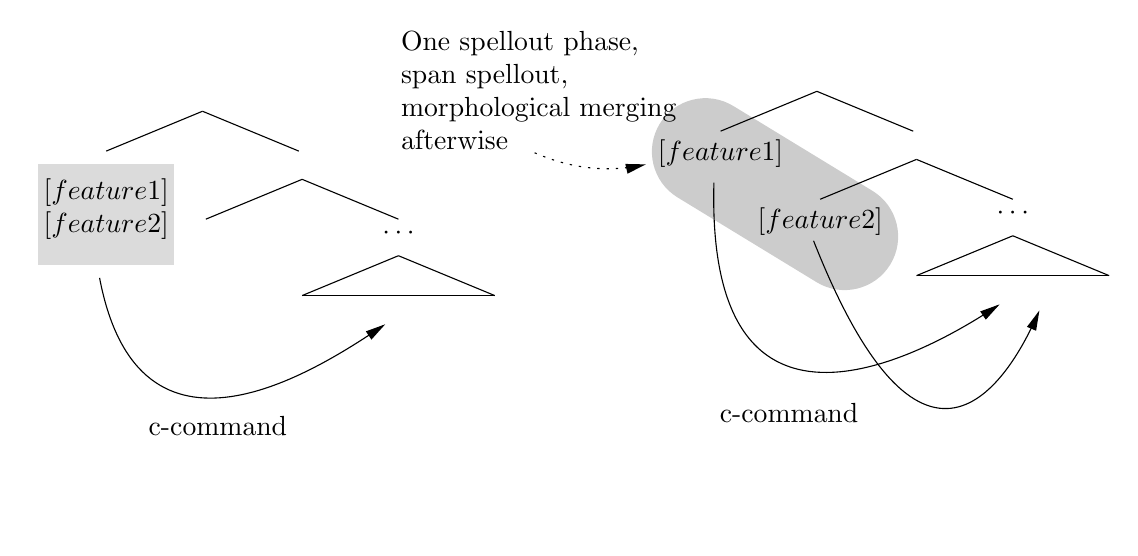
\begin{tikzpicture}[x=0.75pt,y=0.75pt,yscale=-0.8,xscale=0.8]
    %uncomment if require: \path (0,300); %set diagram left start at 0, and has height of 300
    
    %Shape: Rectangle [id:dp9576114178446504] 
    \draw  [draw opacity=0][fill={rgb, 255:red, 74; green, 74; blue, 74 }  ,fill opacity=0.2 ] (29,89) -- (111,89) -- (111,149.33) -- (29,149.33) -- cycle ;
    %Straight Lines [id:da7039895072894264] 
    \draw    (70,81) -- (128,57) ;
    %Straight Lines [id:da7836793109340203] 
    \draw    (186,81) -- (128,57) ;
    %Straight Lines [id:da42956364961038185] 
    \draw    (130,122) -- (188,98) ;
    %Straight Lines [id:da15598911164558582] 
    \draw    (246,122) -- (188,98) ;
    %Straight Lines [id:da5837645378937253] 
    \draw    (188,168) -- (246,144) ;
    %Straight Lines [id:da5024296278135387] 
    \draw    (304,168) -- (246,144) ;
    %Straight Lines [id:da5834640863818097] 
    \draw    (188,168) -- (304,168) ;
    %Curve Lines [id:da2610330987113729] 
    \draw    (66,157.33) .. controls (89.76,282.07) and (195.85,213.73) .. (236.78,186.16) ;
    \draw [shift={(238,185.33)}, rotate = 145.98] [fill={rgb, 255:red, 0; green, 0; blue, 0 }  ][line width=0.08]  [draw opacity=0] (12,-3) -- (0,0) -- (12,3) -- cycle    ;
    %Straight Lines [id:da5872155105544175] 
    \draw    (440,69) -- (498,45) ;
    %Straight Lines [id:da7758281551961919] 
    \draw    (556,69) -- (498,45) ;
    %Straight Lines [id:da9890766953965691] 
    \draw    (500,110) -- (558,86) ;
    %Straight Lines [id:da7429335739442791] 
    \draw    (616,110) -- (558,86) ;
    %Straight Lines [id:da6715636145953721] 
    \draw    (558,156) -- (616,132) ;
    %Straight Lines [id:da3610502824716557] 
    \draw    (674,156) -- (616,132) ;
    %Straight Lines [id:da5763546694322226] 
    \draw    (558,156) -- (674,156) ;
    %Curve Lines [id:da3553221919868479] 
    \draw    (436,100) .. controls (431.05,278.2) and (565.27,201.9) .. (606.77,174.16) ;
    \draw [shift={(608,173.33)}, rotate = 145.98] [fill={rgb, 255:red, 0; green, 0; blue, 0 }  ][line width=0.08]  [draw opacity=0] (12,-3) -- (0,0) -- (12,3) -- cycle    ;
    %Curve Lines [id:da09796494833456726] 
    \draw    (496,135) .. controls (563.97,307.38) and (615.44,214.88) .. (631.3,178.62) ;
    \draw [shift={(632,177)}, rotate = 113.2] [fill={rgb, 255:red, 0; green, 0; blue, 0 }  ][line width=0.08]  [draw opacity=0] (12,-3) -- (0,0) -- (12,3) -- cycle    ;
    %Rounded Rect [id:dp8106345695133526] 
    \draw  [draw opacity=0][fill={rgb, 255:red, 0; green, 0; blue, 0 }  ,fill opacity=0.2 ] (403.35,64.58) .. controls (412.62,49.38) and (432.46,44.57) .. (447.67,53.83) -- (531.48,104.94) .. controls (546.69,114.21) and (551.5,134.04) .. (542.23,149.25) -- (542.23,149.25) .. controls (532.96,164.45) and (513.12,169.26) .. (497.91,159.99) -- (414.1,108.89) .. controls (398.89,99.62) and (394.08,79.78) .. (403.35,64.58) -- cycle ;
    %Curve Lines [id:da07394162000221738] 
    \draw  [dash pattern={on 0.84pt off 2.51pt}]  (328,82) .. controls (350.43,91.75) and (371.9,93.9) .. (393.35,89.36) ;
    \draw [shift={(395,89)}, rotate = 167.2] [fill={rgb, 255:red, 0; green, 0; blue, 0 }  ][line width=0.08]  [draw opacity=0] (12,-3) -- (0,0) -- (12,3) -- cycle    ;
    
    % Text Node
    \draw (70,94.4) node [anchor=north] [inner sep=0.75pt]    {$ \begin{array}{l}
    \left[\text{feature 1}\right]\\
    \left[\text{feature 2}\right]
    \end{array}$};
    % Text Node
    \draw (246,125.4) node [anchor=north] [inner sep=0.75pt]    {$\cdots $};
    % Text Node
    \draw (94,239) node [anchor=north west][inner sep=0.75pt]   [align=left] {c-command};
    % Text Node
    \draw (440,72.4) node [anchor=north] [inner sep=0.75pt]    {$\left[\text{feature 1}\right]$};
    % Text Node
    \draw (616,113.4) node [anchor=north] [inner sep=0.75pt]    {$\cdots $};
    % Text Node
    \draw (438,231) node [anchor=north west][inner sep=0.75pt]   [align=left] {c-command};
    % Text Node
    \draw (500,113.4) node [anchor=north] [inner sep=0.75pt]    {$\left[\text{feature 2}\right]$};
    % Text Node
    \draw (246,7) node [anchor=north west][inner sep=0.75pt]   [align=left] {One spellout phase,\\span spellout,\\morphological merging\\afterwise};
    
    
    \end{tikzpicture}    